
\chapter{手机主题推荐系统整体设计与实现}
    \section{前言}
    小米主题应用拥有成千上万款主题包,而一个用户整个活跃周期只能接触不到十分之一的主题,所以我们现在面临的一个问题是,如何帮助用户发现新的主题,这些主题同时满足俩个条件:1、不能和用户之前看过的、购买过的主题包重复。2、不能和用户之看买过的、购买过的主题不相关,而这也是我们开发的手机主题推荐系统所要达到的目标之一。除此之外,手机主题推荐系统要达到的目标之二是帮助第三方设计师推广其作品。手机主题应用本身既不生产主题包,也不消费主题包,我们的存在价值就是提供一个平台,能让用户、设计师和广告商从中受益。每个设计师都希望更多的用户体验、使用他\\她们的主题,尤其是对于刚出道的设计师。得益于个性化推荐系统的投入使用,我们现在可以把更多的主题包直接推送给那些潜在消费者面前。

    本章节主要介绍如何介绍手机主题推荐系统的完整架构。手机主题推荐由推荐模块、用户画像模型、用户兴趣探索模块组成。推荐过程流程为:首先,推荐系统把用户画像模型中兴趣需求信息和推荐主题模型中的特征信息匹配,然后使用排序算法进行计算筛选找到用户可能感兴趣的推荐主题,最后推荐给用户。
    \section{手机主题推荐系统设计}
    
    \begin{figure}
      \centering
        \framebox{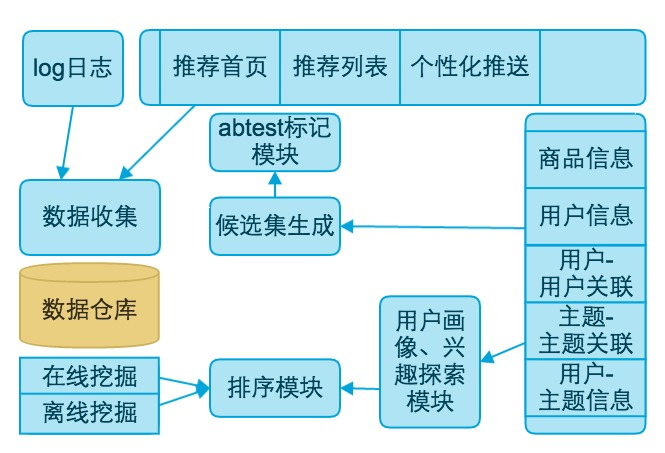
\includegraphics[scale=0.6]{figures/hl_recmd_structure2}}
        \figcaption{推荐系统引擎框架总览图}
        \label{pic:hl_recmd_structure2}
      \end{figure}

    推荐系统框架如\autoref{pic:hl_recmd_structure2}。最顶层显示的是推荐系统对外的服务接口。由于不同展位的输入输出参数差异较大,因此这一层没有做过多的抽象,每个展位有自己特定的接口形式。接口层会调用abtest配置模块,对接入的流量按照uuid、城市等维度进行分流量的配置。Abtest配置模块之下,是推荐候选集的生成,排序和业务处理模块。候选集生成和排序模块,除了针对不同展位有不同逻辑以外,对同一展位的不同策略也有不同的逻辑。abtest模块在配置流量策略的时候,可以根据需要单独配置候选集策略和排序策略。从接口层接受到的每次响应请求会打印一些必要的日志,记录这次请求的一些必要的上下文信息以及用户及item相关的特征信息,以便生成用户行为数据。这些日志通过flume传输到HDFS上面。借助Hadoop、Hive、Spark等平台对原始日志进行处理,从而得到需要的各种数据及模型:包括用户的画像信息,用户之间的相似度,item之间的相似度。在推荐系统的候选集生成这一块,重度使用了传统的user based,item based协同过滤算法,协同过滤算法需要在用户行为较丰富的情况下才能奏效。而对于那些行为稀少的用户,需要根据平台的特点进行做好冷启动策略。这里面需要注意的是,推荐系统引入了时间衰减的因子,从而使新的行为起的作用大于老的行为,从结果来看确实对于效果会有提升。

    \subsection{数据集}
    我们的数据来源有俩部分。1、主动推送,推送有两个特点,一个是异步,可以在用户没有使用APP的时候,将消息推送给他,所以可以作为用户召回的一种手段;另一个是快且实时,因此它也是提高用户活跃度的一种方式。主动推送能够确保优秀的新主题包的时候非常及时的到达用户。2、被动响应,就是用户打开应用,跳转到主题推荐页面,这时才会给用户做推荐。这俩种数据来源都包含着用户行为数据,而用户行为数据是我们的手机主题推荐系统主要驱动数据。用户行为数据包括俩类:隐式反馈数据和显示反馈数据,隐式数据包括用户点击、浏览、搜索关键字等,显示数据主要是用户点赞和评星,显示数据在推荐算法中的权重占比很大,因为如果一个用户给一个主题评星为5星,我们就知道用户确确实实是喜欢这个主题,但是如果用户仅仅是浏览了一款主题,我们是没有办法知道用户真实的想法。通过我们的统计发现,显示数据大约占了1.2\%的比重,隐式数据占了98.8\%的比重,所以我们的推荐系统设计、实现主要是基于隐式用户数据的。

    \subsection{候选集的生成}
    通过用户历史行为数据生成推荐列表,我们把相似的主题包放在候选集中。我们主要利用Item-based Collaborative Filtering算法生成候选集,定义N$_u$表示用户u之前喜欢的主题集合,则用户u对主题i的偏好度根据\autoref{ItemCF}可得,
    \begin{equation}
    p(u,i)=\sum \limits _{j\in N(u)}^{} r(u,j)s(i,j)
    \label{ItemCF}
    \end{equation}

    其中,r$_{u,j}$表示用户u对主题j的偏好度,s$_{i,j}$表示主题i和主题j之间的相似度。Item based Collaborative Filtering算法定义俩个主题之间的相似度由集中在这个俩个主题的用户行为数据计算得出。N$_{i}$为看过主题i的用户集合,N$_{j}$为为看过主题j的用户集合,因此,主题i和主题j的相似度计算公式为\autoref{Item-item-similar}
    \begin{equation}
    s(i,j)=\frac{\left | N(i)\cap N(j) \right |}{\sqrt{\left | N(i) \parallel N(j) \right |}}
    \label{Item-item-similar}
    \end{equation}

    根据\autoref{Item-item-similar}可知,如果有很多用户同时看了主题i和主题j,那么主题i和主题j之间的相似度就会很高,不幸的是,这也会导致所有热门主题与所有主题的相似度都很高。通过A/B测试我们得知,根据用户最近行为作出的推荐比根据用户之前行为作出的推荐,点击转换率比例为1.8:1,因此如果用户最近行为和之前行为有冲突,推荐系统应该倾向于根据用户最近行为作出推荐,而不是反过来。

    \subsection{排序}
    排序之前先过滤掉用户之前接触过的主题包,对于剩余的主题,我们利用生成候选集时得到的用户-主题相关度对主题排序,作为最终推荐结果的重要依据,需要注意的是确保每种类型的主题都要或多或少的推荐一俩款,即保持推荐多样性。最后,推荐结果会对用户给出推荐理由,如一个用户之前买过一款《似水流年》的主题包,我们给他推荐了一款《青春不老 我们不散》的主题,给出的解释是:因为您之前购买过《似水流年》

  \section{用户画像与推荐系统}
  一个好的推荐系统要给用户提供个性化的、高效的、动态准确的推荐,那么推荐系统应能够获取反映用户多方面的、动态变化的兴趣偏好,推荐系统有必要为用户建立一个用户兴趣探索模型,该模型能获取、表示、存储和修改用户兴趣偏好,能进行推理,对用户进行分类和识别,帮助系统更好地理解用户特征和类别,这就是我们要引进用户画像的根本原因。用户画像模块和兴趣探索模块的关系如\autoref{pic:hl_iterate}所示。
  \begin{figure}
    \centering
      \framebox{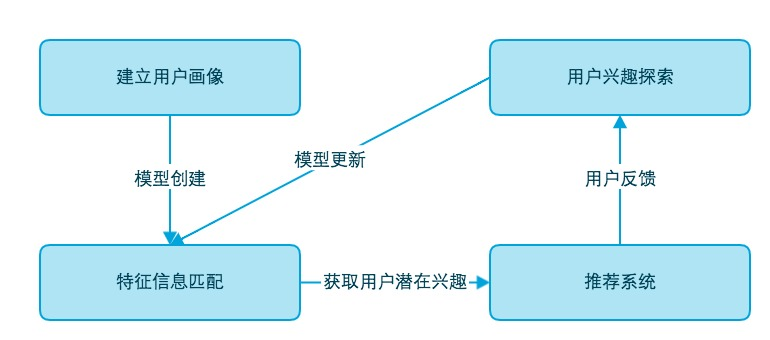
\includegraphics[scale=0.4]{figures/hl_iterate}}
      \figcaption{用户画像架构示意图}
      \label{pic:hl_iterate}
  \end{figure}

  利用用户的画像,结合时间、天气等上下文信息,给用户做一些更加精准化的推荐是一个不错的方向。推荐系统根据用户画像进行推荐,所以用户画像对推荐系统的质量有至关重要的影响。建立用户画像模型之前需要考虑问题有:模型的输入数据有哪些,如何获取模型的输入数据;如何考虑用户的兴趣及需求的变化;建模的对象是谁以及如何建模;模型的输出是什么。用户画像模型的输入数据主构成包括:
  \begin{itemize}
  \item 用户属性,分为社会属性和自然属性,包括用户最基本的如用户的姓名、年龄、职业、收入、学历等信息。用户注册时的对自然属性和社会属性进行初始建模。 
  \item 用户手工输入的信息:是用户主动输出给系统的信息,包括用户在搜索引擎中打出的关键词,用户评论中发布的感兴趣的主题、频道。还有一类重要的信息就是用户反馈的信息,包括用户自己对推荐结果的满意程度;用户标注的浏览页面的感兴趣、不感兴趣或感兴趣的程度等。
  \item 用户的浏览行为和浏览内容:用户浏览的行为和内容体现了用户的兴趣和需求,它们包括浏览次数、频率、停留时间等,浏览页面时的操作(收藏、保存、复制等)、浏览时用户表情的变化等。服务器端保存的日志记录了用户的浏览行为和内容。
  \end{itemize}

  手机主题推荐系统对每个新注册用户会生成一个用户画像,刚开始只是包含最基本的用户人口信息,在维护过程中会逐渐增加用户行为和行为偏好,然后利用离线训练模型生成用户喜好的主题,详细内容将在第四章、第五章展开。
  \section{量化评估推荐系统}
  

  \section{本章小结}
  我们的手机主题推荐系统还遇到一种情况是,有时候推荐时,排序较高的主题不一定是用户需要的,而排序较低的主题有可能是用户期望看到的。例如,一个用户喜欢读弗洛伊德的《梦的解析》,那么他有可能会喜欢《异梦空间》这款主题,但是这款主题很冷门,推荐系统没办法挖掘出其价值。再比如,像《似水流年》这样常月霸占免费排行榜第一、第二位置的热门主题包,我们实际上是不需要对其作任何推广、推荐的。除此之外,我们也希望手机推荐系统能推陈出新,而不是一成不变。为了解决这些问题,本人基于手机主题推荐系统开发了用户画像功能模块和用户兴趣功能模块。